\clearpage
\section{Diffusion Distance}

The diffusion distance is given by $\sqrt{Dt}$, which is found in the equation that is used to describe the concentration after a time $t$ in a thin layer of the diffusing species is concentrated at $x=0$ of a semi-infinte sample \cite{diff}:
\begin{align}
  \label{eq:3}
  c(x,t)&=\dfrac{M}{\sqrt{\pi D t} \exp\left(-\dfrac{x^2}{4DT}\right)}.
\end{align}

Using the previous statement, the difussion distance was calculated using a time range from zero to (tengo que arreglar esta parte, porque creo que meti la pata con el calculo del tiempo :c). The plots for the diffusion distance as a function of time and the lilnealization of the diffusion distance are shown in the figure \ref{fig:length}.

\begin{figure}[h]
 \centering
 \captionsetup{justification=centering}
  \subfloat[]{
   \label{fig:l}
    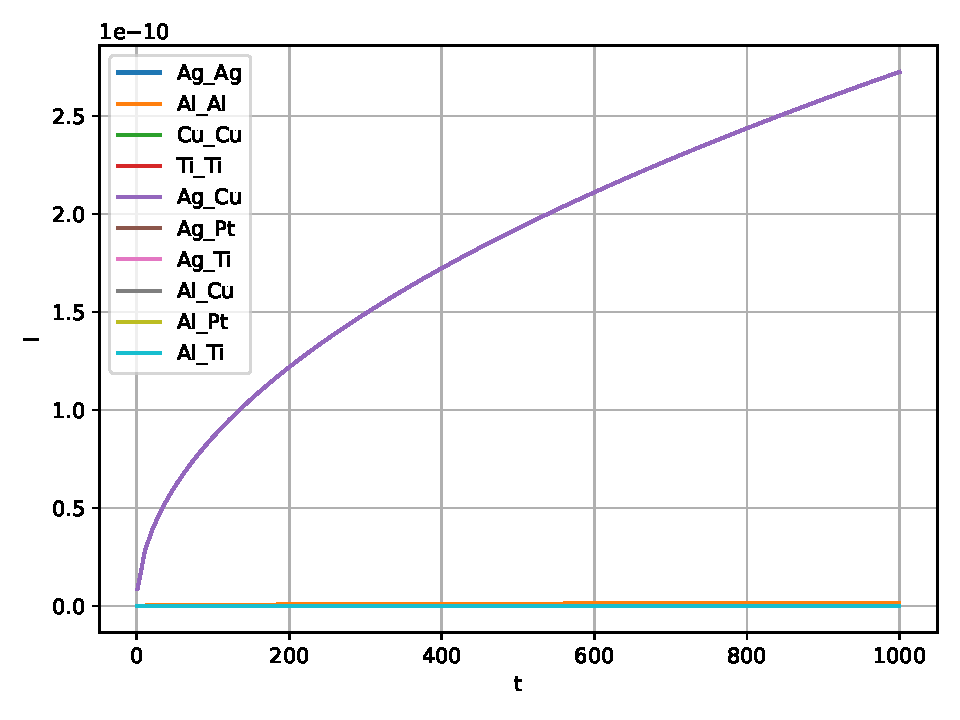
\includegraphics[width=0.5\textwidth]{graficas/l.pdf}}
  \subfloat[]{
   \label{fig:log_l}
    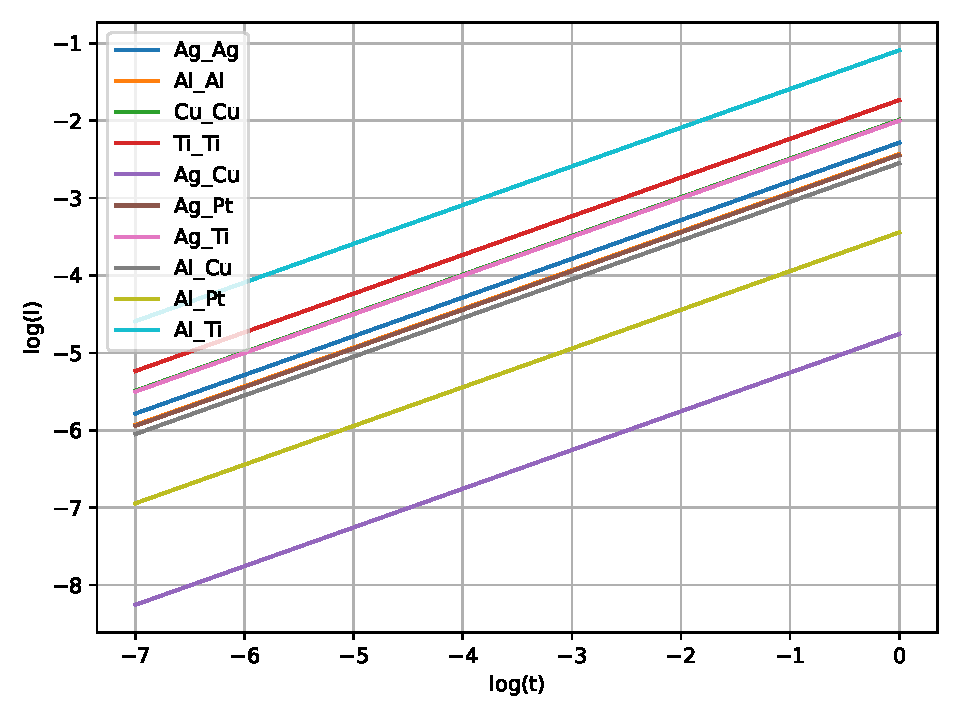
\includegraphics[width=0.5\textwidth]{graficas/log(l).pdf}}
 \caption{a) Diffusion distance $x$ (m) as a function of time $t$ (s) and b) logarithm of the diffusion distance $log(x)$ as a function of time $t$ ($s$). \\
 \textit{Source: Data from \citep{kakusan}, visualization by the author (code available at \citep{mygit}).}}
 \label{fig:length}
\end{figure}


\subsection{Self-diffusion}

The shoshfdos

\begin{figure}[H]
 \centering
 \captionsetup{justification=centering}
  \subfloat[]{
   \label{fig:dist_ag}
    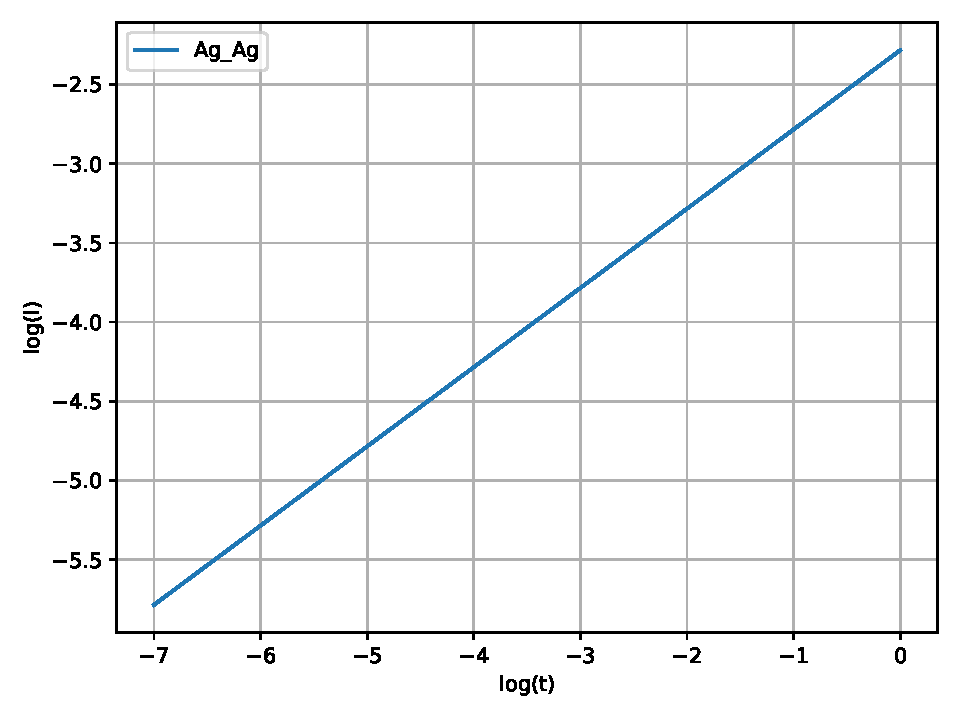
\includegraphics[width=0.5\textwidth]{graficas/Ag_Ag_log(l).pdf}}
  \subfloat[]{
   \label{fig:dist_al}
    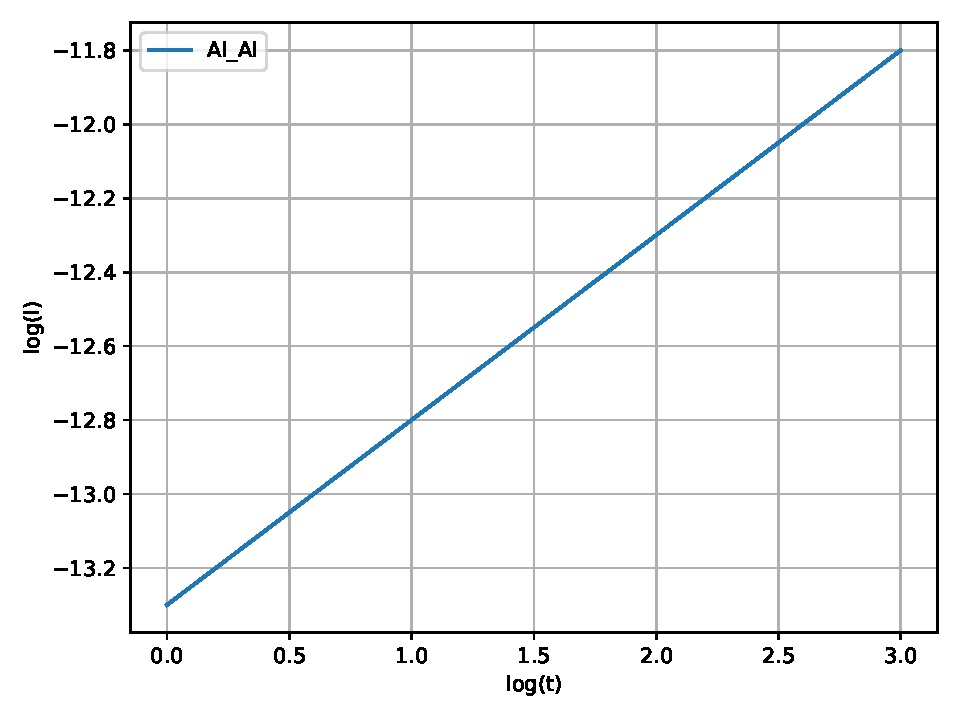
\includegraphics[width=0.5\textwidth]{graficas/Al_Al_log(l).pdf}} \\
  \subfloat[]{
   \label{fig:dist_cu}
    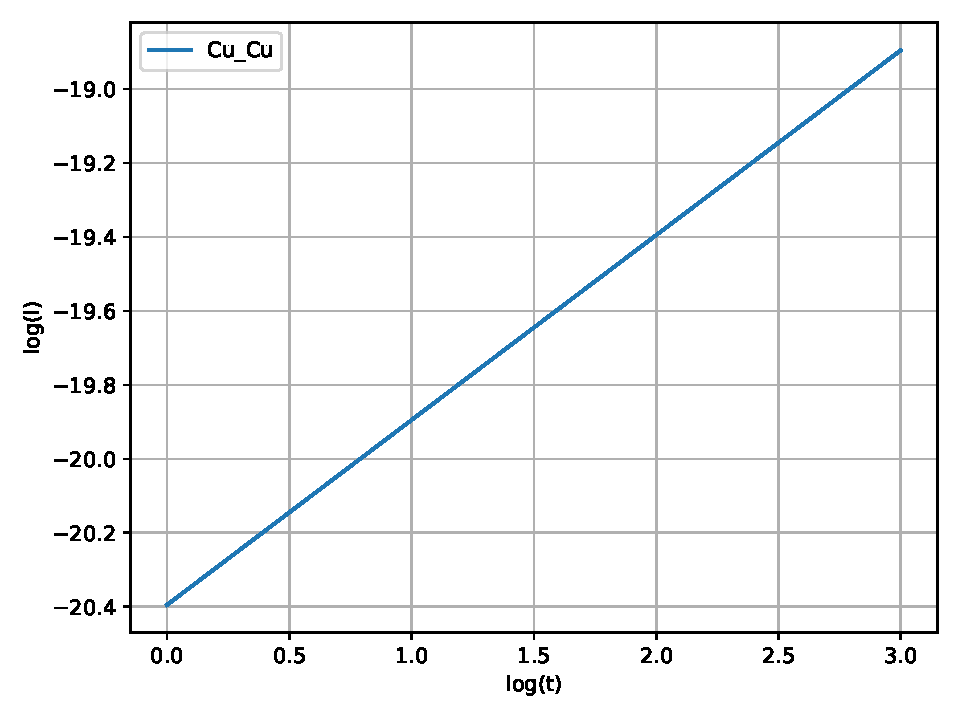
\includegraphics[width=0.5\textwidth]{graficas/Cu_Cu_log(l).pdf}}
  \subfloat[]{
   \label{fig:dist_ti}
    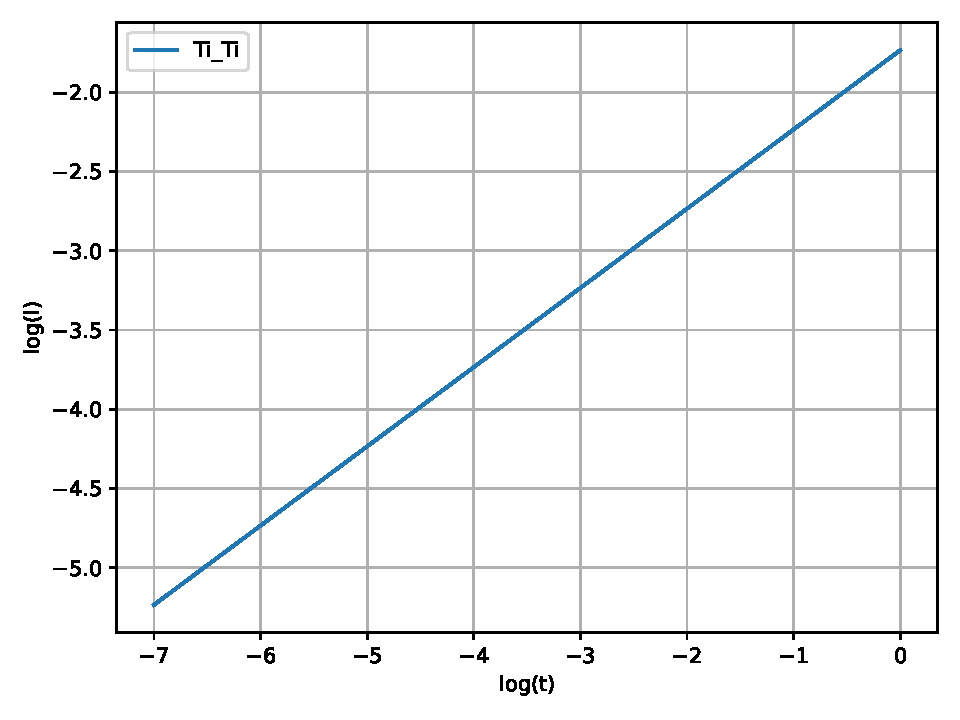
\includegraphics[width=0.5\textwidth]{graficas/Ti_Ti_log(l).pdf}}
 \caption{Distance of diffusion : a) silver, b) aluminum, c) copper and d) titanium.\\ 
 \textit{Source: Data from \citep{kakusan}, visualization by the author (code available at \citep{mygit}).}}
 \label{fig:selfdiff_dist}
\end{figure}


\subsection{Solute diffusion}

The fsdfojsofdjsodfs

\begin{figure}[H]
 \centering
 \captionsetup{justification=centering}
  \subfloat[]{
   \label{fig:dist_ag_cu}
    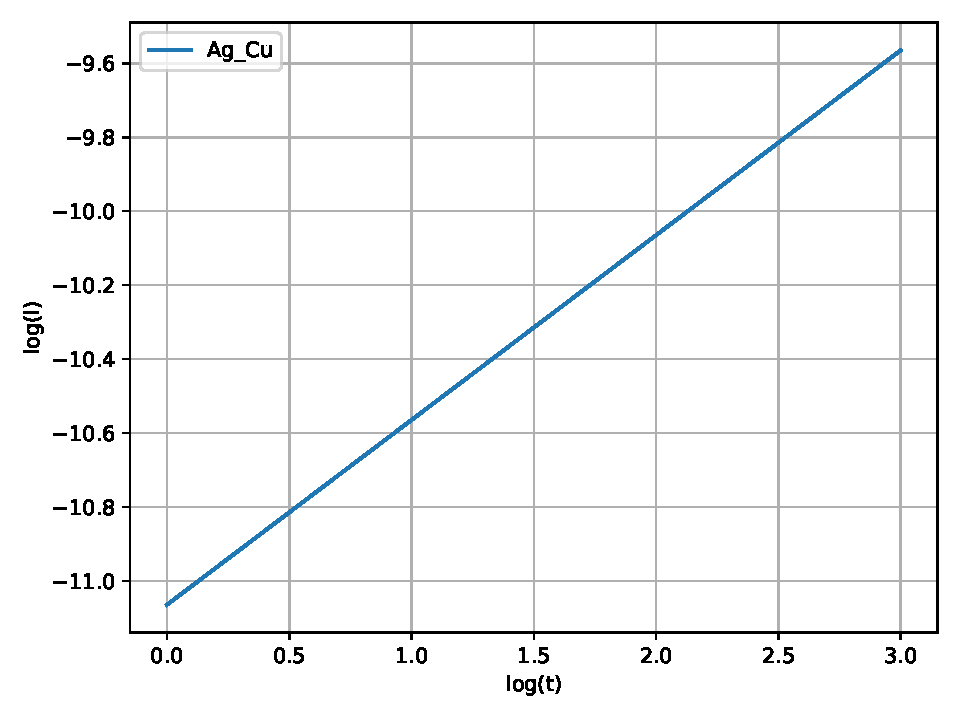
\includegraphics[width=0.5\textwidth]{graficas/Ag_Cu_log(l).pdf}}
  \subfloat[]{
   \label{fig:dist_al_cu}
    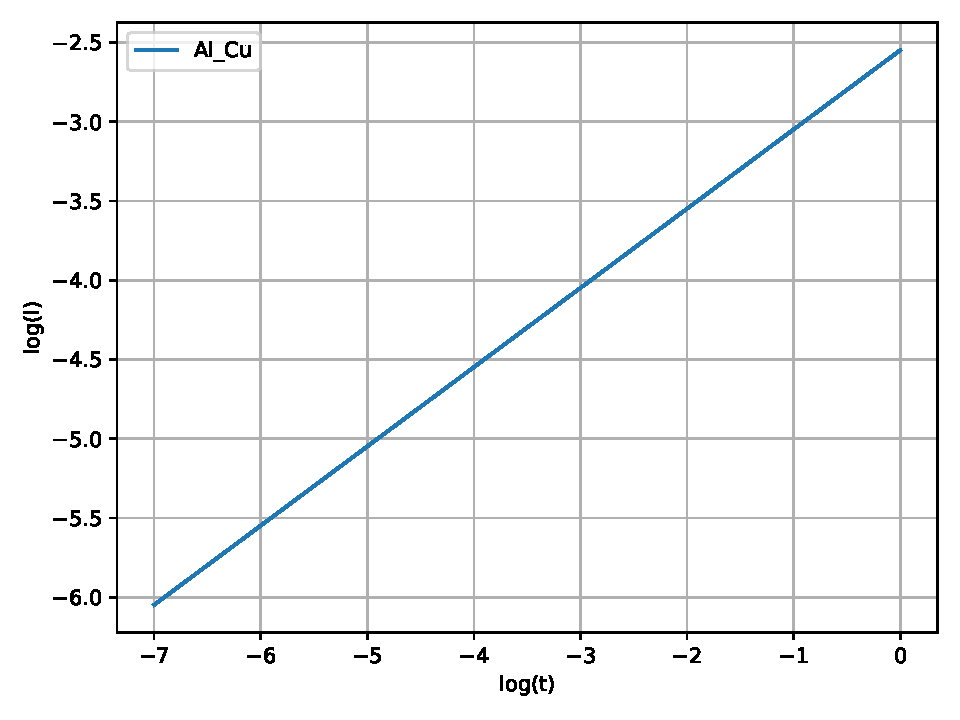
\includegraphics[width=0.5\textwidth]{graficas/Al_Cu_log(l).pdf}} \\
  \subfloat[]{
   \label{fig:dist_ag_pt}
    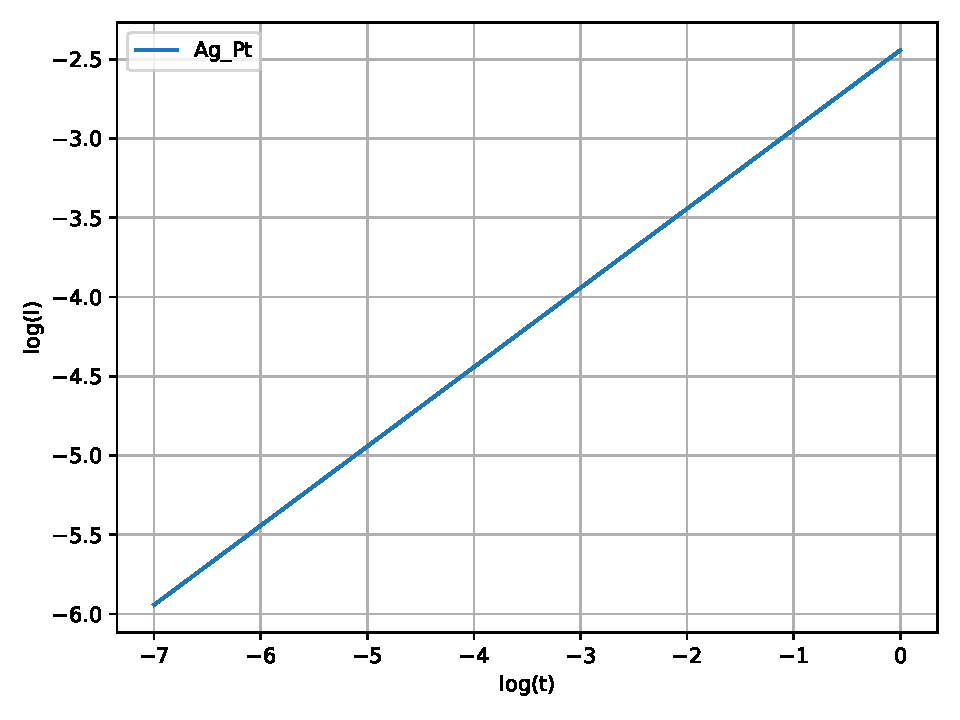
\includegraphics[width=0.5\textwidth]{graficas/Ag_Pt_log(l).pdf}}
  \subfloat[]{
   \label{fig:dist_al_pt}
    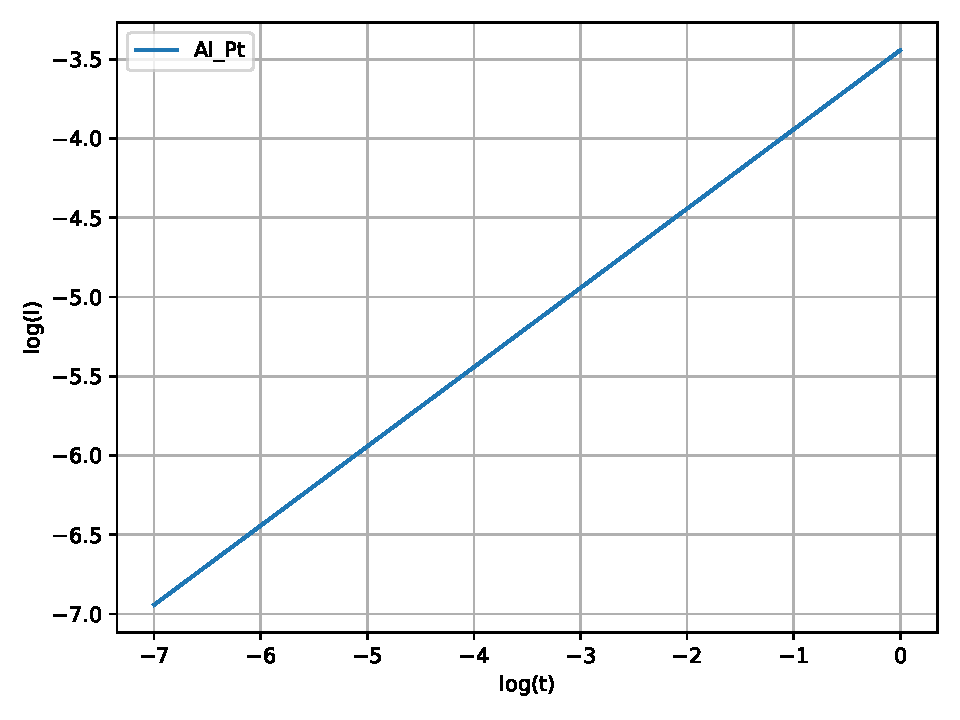
\includegraphics[width=0.5\textwidth]{graficas/Al_Pt_log(l).pdf}} \\
  \subfloat[]{
   \label{fig:dist_ag_ti}
    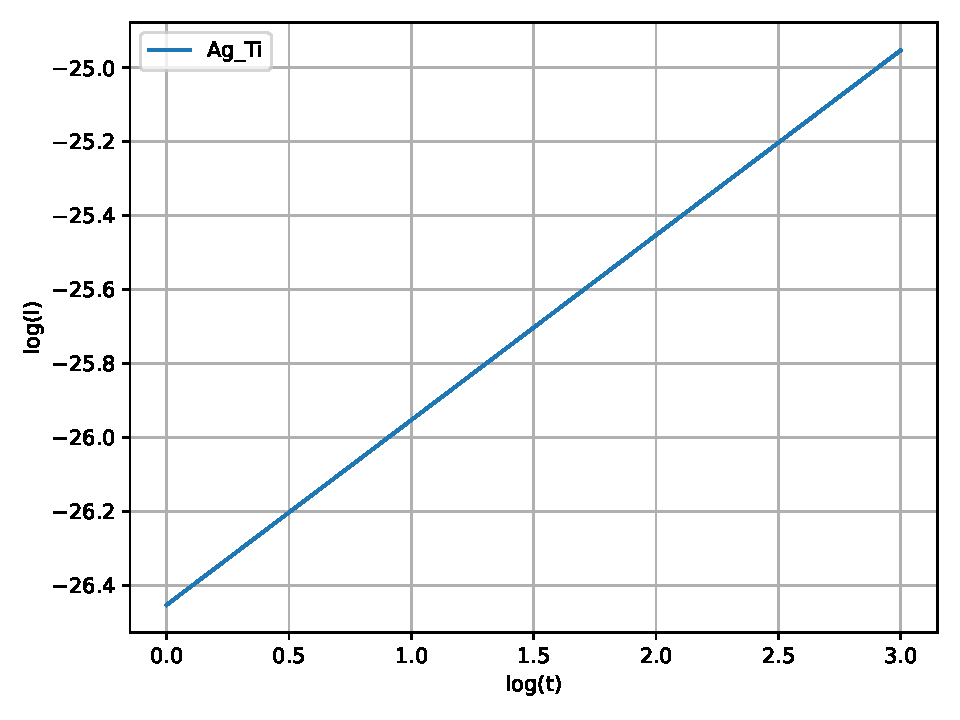
\includegraphics[width=0.5\textwidth]{graficas/Ag_Ti_log(l).pdf}}
  \subfloat[]{
   \label{fig:dist_al_ti}
    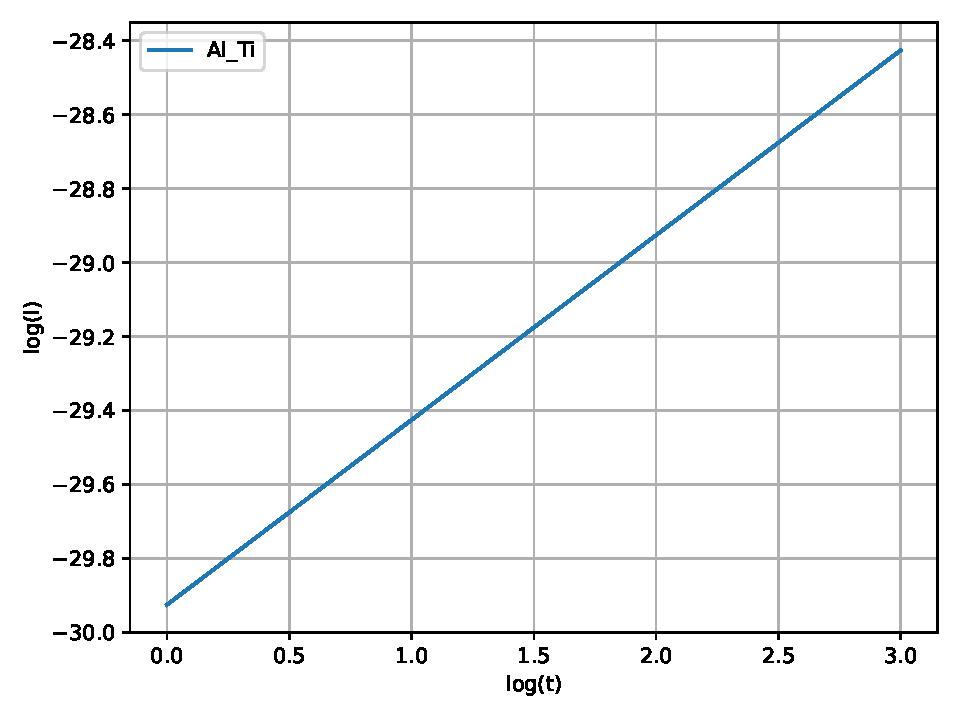
\includegraphics[width=0.5\textwidth]{graficas/Al_Ti_log(l).pdf}}
 \caption{Diffusion distance fjosjdfosjfos.\\ 
 \textit{Source: Data from \citep{kakusan}, visualization by the author (code available at \cite{mygit}).}}
 \label{fig:diff_dist}
\end{figure}
